% =============================================================
% Materials and Methods -- DINOcow paper
% Order and team-written sections follow PaperDINOcow.pdf. The model, evaluation,
% baselines and implementation subsections come from the previous methods.tex
% (76-cow version); the PDF lacked the evaluation part that Results relies on.
% =============================================================
\section{Materials and Methods}
\label{sec:methods}

\subsection{Study area and data acquisition}
\label{sec:data}

The study was conducted at the Experimental Agricultural Field of Tecnológico de Monterrey (CAETEC), located in Querétaro, Mexico.
Images were collected using an acquisition system installed near the exit of the robotic milking area in pen 6, which houses fresh cows, cows near dry off, and cows starting at two days open.
The system consisted of a Logitech C920 webcam \mJ{(Logitech, Lausanne, Switzerland)} and an ARD-315 passive infrared (PIR) motion sensor \mJ{(Steren, Mexico City, Mexico)}.
The camera was installed in a fixed overhead position to capture the rear dorsal view of cows as they left the milking area (Figure~\ref{fig:camera})\mP{, from May to July 2025}.

\begin{figure}[!htbp]
  \centering
  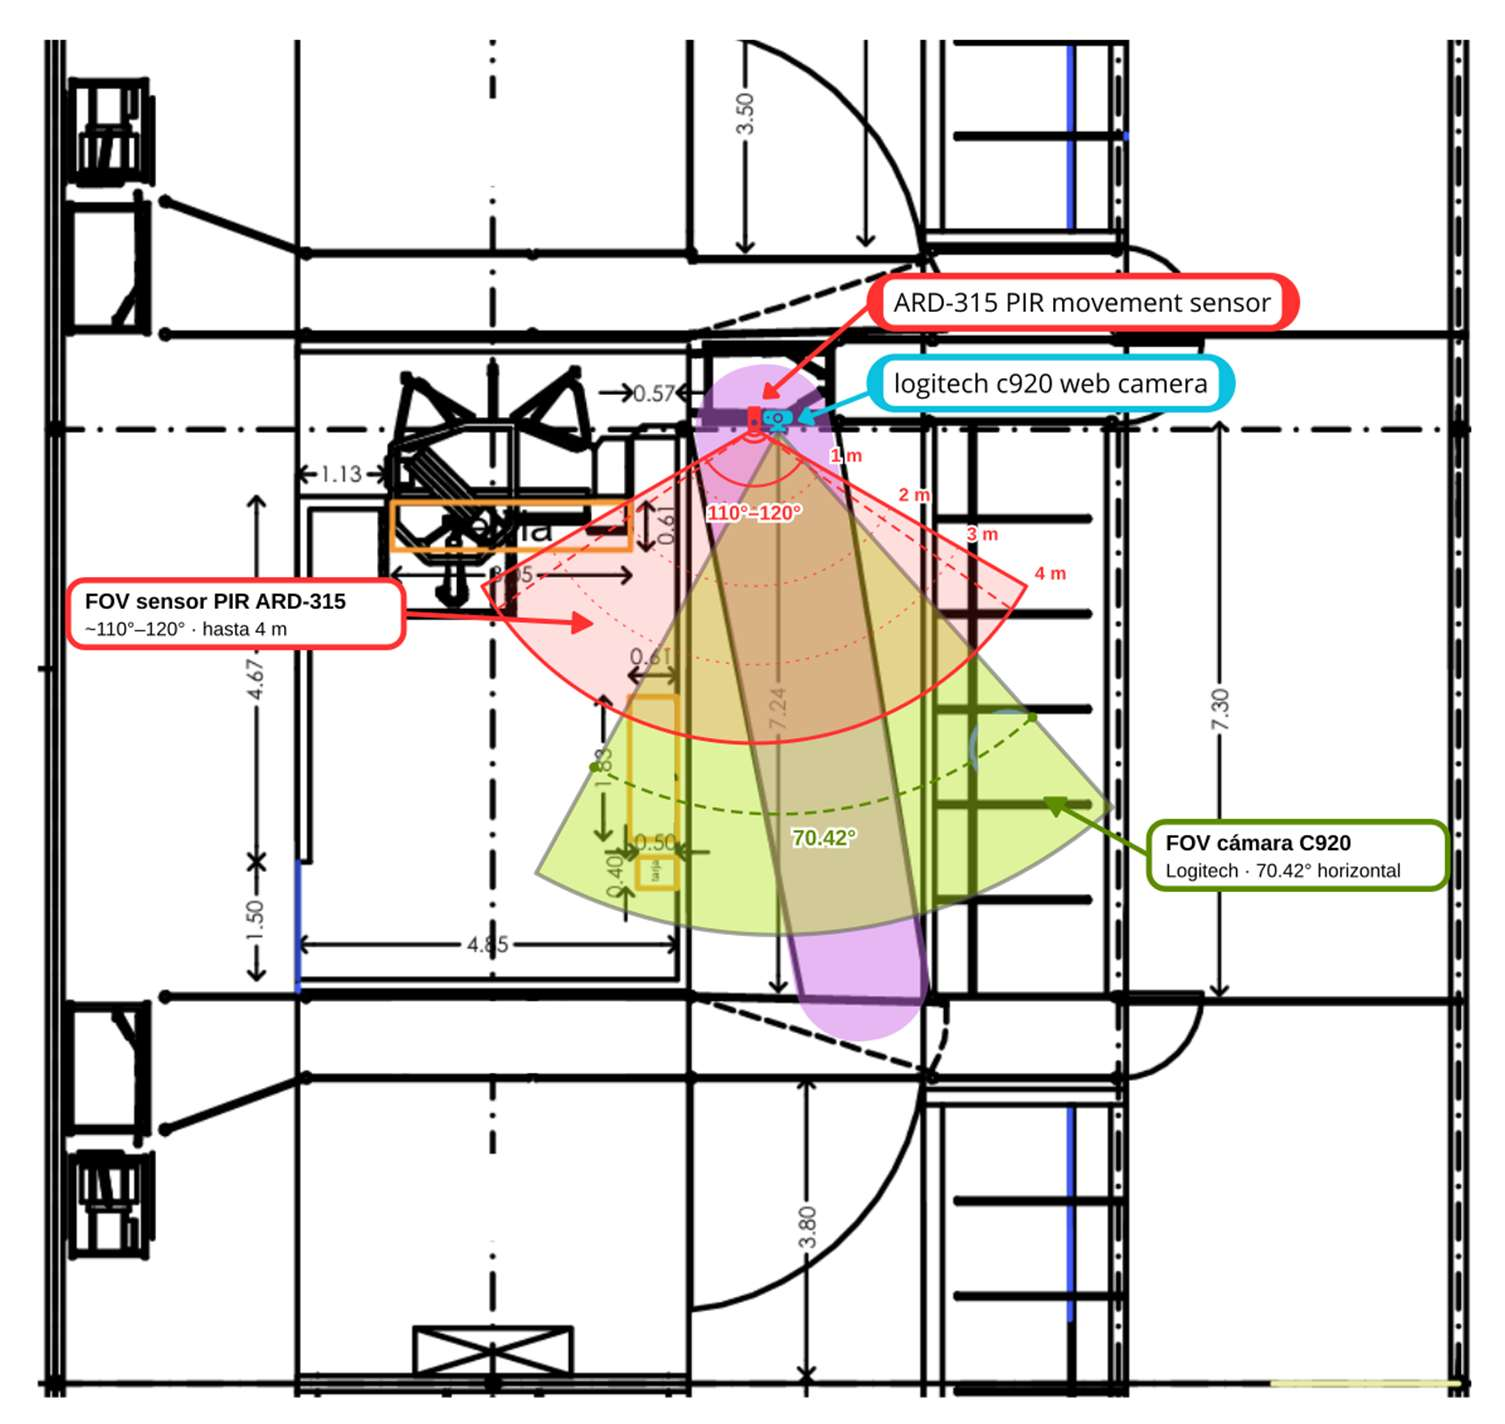
\includegraphics[width=0.55\linewidth]{../figures/word/camara.jpg}
  \caption{\mE{Diagram of the area around the milking robot exit in pen 6, with the corridor (purple), the detection field of the PIR motion sensor (red) and the field of view of the webcam (green).}}
  \label{fig:camera}
\end{figure}

After milking, cows passed through a corridor next to the exit (shown in purple in Figure~\ref{fig:camera}).
A passive infrared (PIR) motion sensor (Steren ARD-315; detection field shown in red) was mounted above the corridor, together with a Logitech C920 webcam (field of view shown in green).
The camera streamed continuously at 1080p ($1920\times1080$ pixels) and 30 frames per second, and when an animal entered the sensor detection area, the sensor triggered the capture of a single frame from the stream.
This arrangement allowed images to be collected automatically from a consistent camera position without requiring additional handling of the animals.

\pendiente{Camera mounting height and angle; how each frame was linked to a cow (robot exit records?); how the dorsal crops were produced (manual or detector).}

\subsection{Image filtering and cleaning}

The 57,780 acquired images were subjected to automated and manual filtering to guarantee visual quality and anatomical relevance for BCS estimation.
In the first phase, images with inadequate brightness were eliminated by grayscale analysis with OpenCV.
Subsequently, following a technique similar to that of \citet{ali2025}, an object detection model based on YOLOv8m pretrained on the COCO dataset automatically discarded images that did not contain a cow.
Examples of both filtering steps are shown in Table~\ref{tab:filtering}.

\begin{table}[!htbp]
  \centering
  \caption{Examples of the first two filtering steps.}
  \label{tab:filtering}
  \begin{tabular}{>{\raggedright\arraybackslash}p{3.6cm}cc}
    \toprule
    Purpose & Images kept & Examples of discarded images \\
    \midrule
    Remove images with more than 80\% dark pixels & 57,780 $\rightarrow$ 47,082 & \raisebox{-0.5\height}{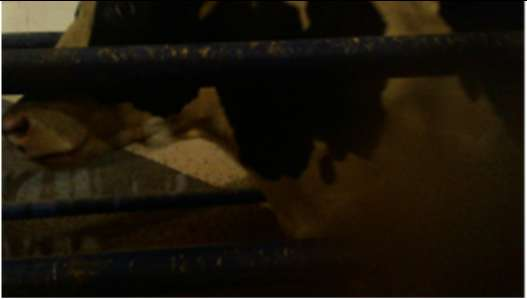
\includegraphics[width=3.4cm]{../figures/word/filtro_oscuras.jpg}} \\[1.2cm]
    Remove images without cows (YOLOv8) & 47,082 $\rightarrow$ 9,213 & \raisebox{-0.5\height}{\shortstack{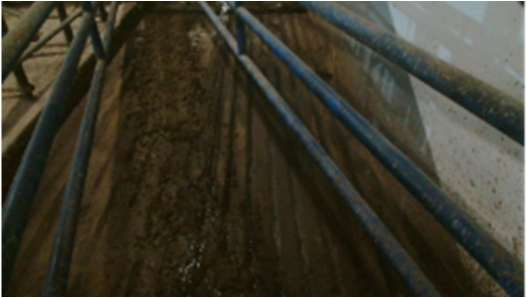
\includegraphics[width=3.4cm]{../figures/word/filtro_sinvaca_a.jpg}\\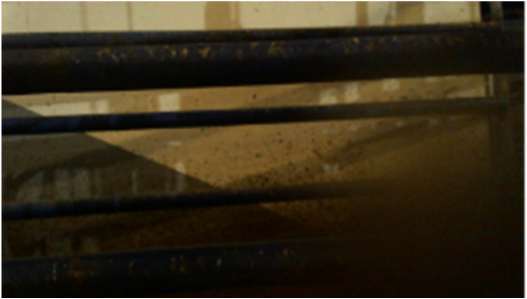
\includegraphics[width=3.4cm]{../figures/word/filtro_sinvaca_b.jpg}}} \\
    \bottomrule
  \end{tabular}
\end{table}

\subsection{Data preparation and cleaning}

Images with poorly captured animals were pre-processed, and images with missing cows or more than one cow were deleted from the dataset with the tools listed in \mbox{Table~\ref{tab:tools}}, on the computer described in Table~\ref{tab:computer}.

\begin{table}[!htbp]
  \centering
  \caption{Tools used and their main purpose.}
  \label{tab:tools}
  \begin{tabularx}{\textwidth}{>{\raggedright\arraybackslash}p{2.8cm}>{\raggedright\arraybackslash}p{4.4cm}X}
    \toprule
    Component & Tool & Purpose \\
    \midrule
    Data collection & Logitech C920, ARD-315 PIR, Raspberry Pi & Collecting the raw images \\
    Model & PyTorch & Training, validation and use of segmentation and BCS models \\
          & Docker & Containers to train, validate and run the models \\
    Version control & Git, GitHub & Collaborative development and tracking of changes \\
    Data annotation & Roboflow & Segmentation of the anatomical regions for BCS \\
    \bottomrule
  \end{tabularx}
\end{table}

\begin{table}[!htbp]
  \centering
  \caption{Computer used for all experiments}
  \label{tab:computer}
  {\begin{tabular}{lll}
    \toprule
    & Component & Details and version \\
    \midrule
    Hardware & CPU & AMD Ryzen 5 5600G, 6 cores, 12 threads \\
             & RAM & 46 GB \\
             & GPU & NVIDIA GeForce RTX 2080, 8 GB of VRAM (driver 595.99) \\
    Software & Operating system & Ubuntu 24.04.5 LTS, kernel 7.0.0-42 \\
             & Docker & 29.9.3 \\
             & Python & 3.10.12 \\
             & PyTorch & 2.9.1 with CUDA 12.6 and cuDNN 9.1 \\
             & timm & 1.0.22 \\
             & NumPy & 2.2.6 \\
             & scikit-learn & 1.7.2 \\
             & Ultralytics & 8.3.150 \\
    \bottomrule
  \end{tabular}}
\end{table}

In the final phase of cleaning, a manual review eliminated images of cows that did not show the anatomical features necessary for a BCS evaluation (ileal region, ischial region, tail base, ribs and spine, and ileal-ischial connection), along with blurry or obstructed images.
After this process, 670 valid images of 76 cows remained, selected with the criteria in Table~\ref{tab:criteria}.

\newcommand{\ej}[1]{\raisebox{-0.5\height}{\includegraphics[width=2.9cm,height=2.4cm,keepaspectratio]{../figures/word/#1.jpg}}}
\begin{table}[!htbp]
  \centering
  \caption{Image selection criteria applied during cleaning.}
  \label{tab:criteria}
  \renewcommand{\arraystretch}{1.1}
  \begin{tabular}{>{\raggedright\arraybackslash}p{5.2cm}cc}
    \toprule
    Criterion & Discarded & Accepted \\
    \midrule
    \textbf{Darkness.} The cow must be distinguishable from the objects around it at once. & \ej{sel_oscuridad_no} & \ej{sel_oscuridad_si} \\[1.3cm]
    \textbf{Brightness.} The body and its critical parts must be visible to the naked eye. & \ej{sel_brillo_no} & \ej{sel_brillo_si} \\[1.3cm]
    \textbf{View.} The image must come from the top camera and show the rear of the cow. & \ej{sel_vista_no} & \ej{sel_vista_si} \\[1.3cm]
    \textbf{Noise.} The animal must be clearly seen. & \ej{sel_ruido_no} & \ej{sel_ruido_si} \\[1.3cm]
    \textbf{Absence of an animal.} The animal must appear in the photograph. & \ej{sel_ausencia_no} & \ej{sel_ausencia_si} \\[1.3cm]
    \textbf{Absence of relevant features.} The sacral and coccygeal bones must be visible to assess body condition. & \ej{sel_rasgos_no} & \ej{sel_rasgos_si} \\
    \bottomrule
  \end{tabular}
\end{table}

\subsection{Instance segmentation and annotation}

To make use of the small dataset of 76 cows, 40 images were selected to train the region segmenter, which then placed pseudo-labels on the remaining images.
The 40 images were annotated by instance segmentation in Roboflow using the body landmarks (ileal region, ischial region, tail base, ribs and spine, and ileal-ischial connection), as illustrated in Figure~\ref{fig:annotation}.
Pseudo-labels have been used before for non-contact monitoring of cattle \citep{qiao2022}.

\begin{figure}[!htbp]
  \centering
  \figthurl{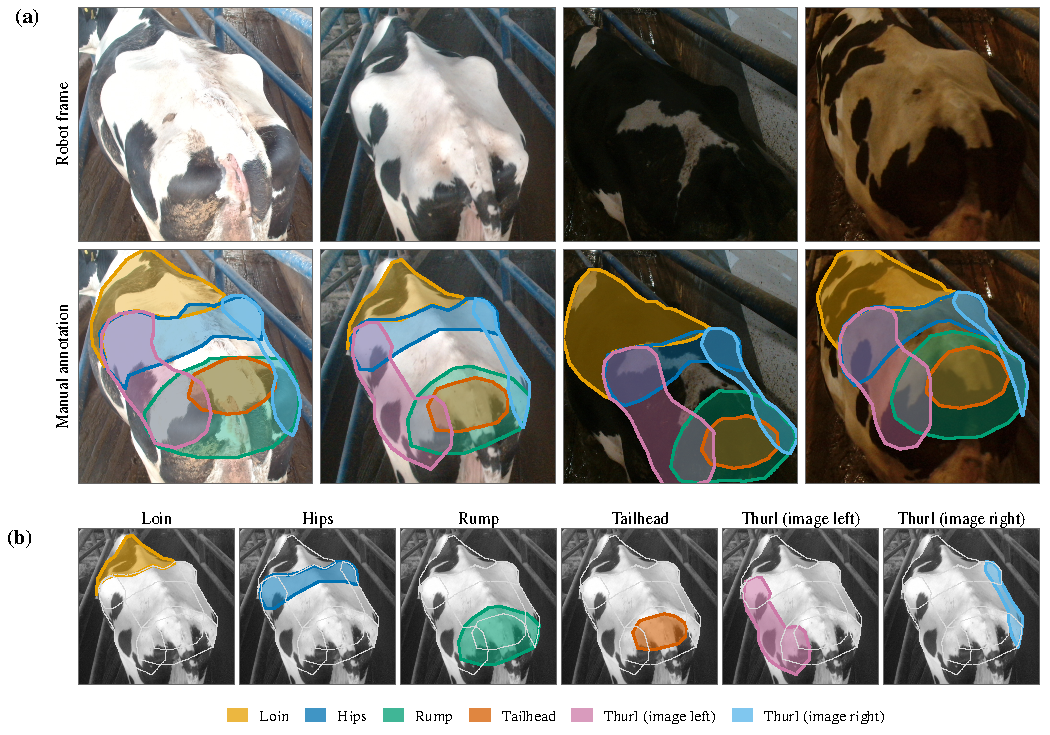
\includegraphics[width=0.97\textwidth]{../figures/segmentation_examples.pdf}}
  \caption{Manual region annotations on robot frames. (a) Four examples. (b) One frame, region by region.}
  \label{fig:annotation}
\end{figure}

\subsection{Labeling BCS}

The images were collected over 52 days (25 May to 15 July 2025), and each image was labeled with a BCS on the 1 to 5 scale, following the decision tree in Figure~\ref{fig:tree}.
From the rear, as in our images, the scorer first judges whether the rump is V- or U-shaped and then how visible the hooks, pins, sacral and sacrococcygeal ligaments and short ribs are.

\begin{figure}[!htbp]
  \centering
  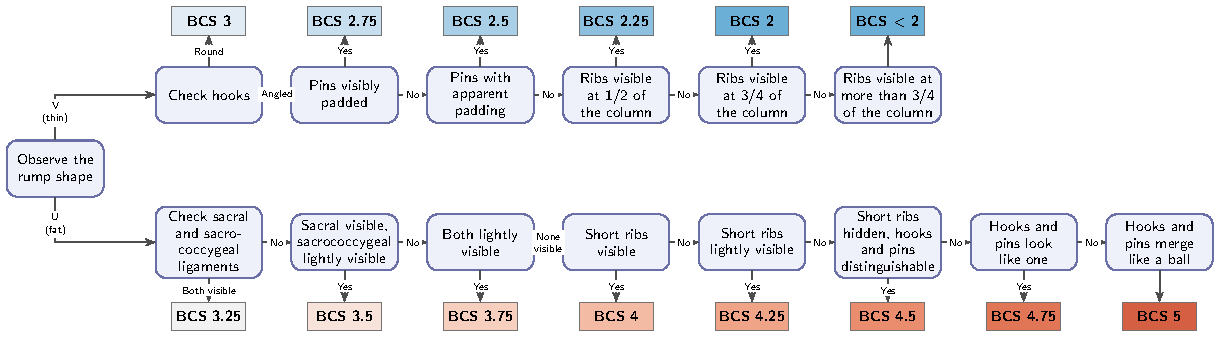
\includegraphics[width=\textwidth]{../figures/arbol_bcs.pdf}
  \caption{Decision tree for scoring BCS from the rear of the cow, adapted from \citet{ferguson1994}. The shape of the rump separates thin (V) from fat (U) cows, and the visibility of the bony landmarks then sets the score in 0.25 steps.}
  \label{fig:tree}
\end{figure}

Subsequently, each score was evaluated independently by two veterinarians with field experience in body condition scoring, whose scores differed from the initial scoring by \mJ{a mean absolute difference of 0.35} BCS points.
This matches the variability between evaluators reported by \citet{ferguson1994}, where experienced observers agreed only 58.1\% of the time.

The resulting dataset holds 670 images of 76 cows, scored from 2.0 to 5.0 in 0.25 steps (mean 3.67, SD 0.99), distributed as shown in Figure~\ref{fig:bcs_dist}, where cows scored more than once count once per score (79 cow--score pairs).
Two cows were scored more than once, one in three months (4.25, 4.0 and 3.5) and another twice, 4.5 between 26 May and 8 June\mP{ 2025} and 2.25 between 24 and 26 June\mP{ 2025}, after she fell ill and lost condition quickly.
Each of their images takes the score of the period in which it was taken, and each animal stays a single group in every split.
The number of images per cow is very uneven, from 1 to 85 (median 5), so a cow photographed often could dominate any image-level average, and we therefore report every result per cow as well.

\begin{figure}[!htbp]
  \centering
  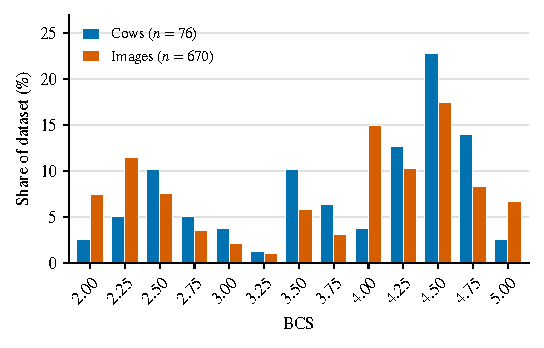
\includegraphics[width=0.62\textwidth]{../figures/bcs_distribution.pdf}
  \caption{BCS distribution in the dataset, as a percentage of cows and of images.}
  \label{fig:bcs_dist}
\end{figure}

\subsection{Image augmentation}

Data augmentation was investigated as a strategy to increase the variability of the training data without requiring additional labeled images.
Based on established image augmentation methods \citep{shorten2019} and their application to automated BCS estimation \citep{yao2026}, a set of geometric and photometric transformations was selected.
These included horizontal flipping, brightness and contrast adjustments, rotation, translation, scaling, and Gaussian noise.
The transformations were evaluated individually and combined to examine their contribution to BCS estimation while preserving the anatomical characteristics relevant to body condition assessment.

Horizontal flipping was applied with a probability of 0.5, while brightness and contrast were varied by $\pm5\%$ and $\pm10\%$.
Geometric transformations were restricted to rotations of $\pm5^\circ$, translations of $\pm3\%$ of the image dimensions, and scaling factors between 0.97 and 1.03.
Gaussian noise was also considered, with a standard deviation of 0.02 relative to the normalized image intensity range.
For each training image, three augmented versions were generated with the same BCS label as the original image.
When geometric transformations were applied, the anatomical masks were adjusted accordingly, and for horizontal flipping the left and right \thurlhl{thurl} regions were also exchanged to keep their correct positions.
Data augmentation was applied only to the training images, while validation and testing used the original images.
In addition, the dataset was divided by cows so that images of the same animal were not shared between training and evaluation.

\pendiente{DINOcow uses no augmentation (ridge on frozen descriptors), and the fine-tuned baselines use different settings (flip, $\pm10^\circ$, $\pm5\%$ shift, scale 0.9--1.1, brightness and contrast 0.2, saturation 0.1, no noise, no $\times3$ copies). Which experiment does this subsection describe? Remove it or state its results.}

\subsection{The DINOcow model}
\label{sec:model}

\mP{Previous 2D models estimate BCS from the whole image or from a single crop of the cow \mbox{\citep{dandil2024,zheng2024,liu2025,yao2026}}, so the network must find by itself which parts of the body carry the information.}
A human scorer does not judge a cow as one single body. BCS charts ask the scorer to look at specific bony landmarks and at how much tissue covers them \citep{edmonson1989,ferguson1994}.
\mP{DINOcow imitates the human scorer in} the three steps shown in Figure~\ref{fig:model}.
It first finds the anatomical regions that scorers inspect \mR{(see \mbox{\textit{\nameref{sec:segmentation}}})}, then describes the appearance of each region with a general-purpose vision model that has never seen a cow's score \mR{(see \mbox{\textit{\nameref{sec:features}}})}, and finally learns a single linear map from those descriptions to BCS \mR{(see \mbox{\textit{\nameref{sec:ridge}}})}.
Only this last step uses BCS labels, which keeps the number of parameters fitted to the 76 cows small, 5125 coefficients and an intercept, against millions of weights for the networks fine-tuned end to end that we compare with \mR{(see \mbox{\textit{\nameref{sec:baselines}}})}.

\begin{figure}[!htbp]
  \centering
  \figthurl{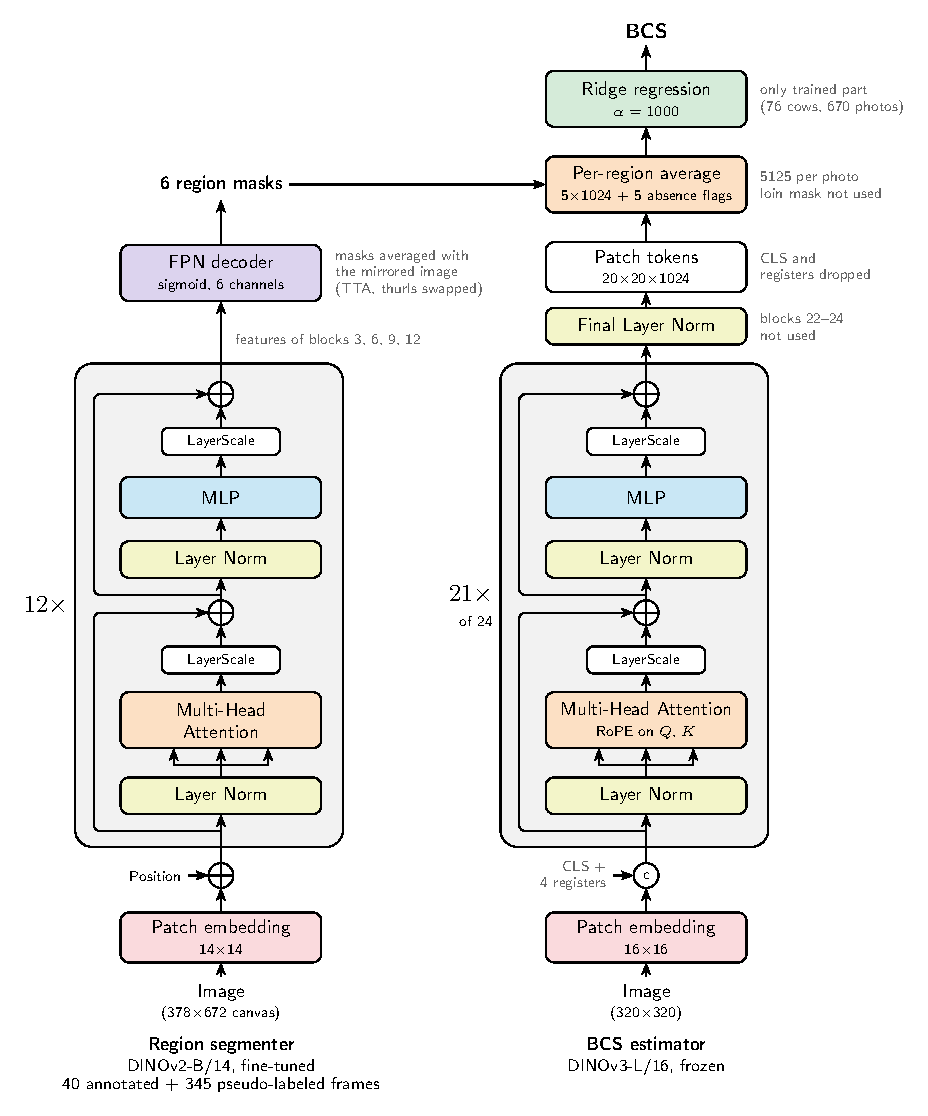
\includegraphics[width=0.75\linewidth]{../figures/main_model.pdf}}
  \caption{DINOcow model architecture, with the region segmenter (left) and the BCS estimator (right).}
  \label{fig:model}
\end{figure}

\subsubsection{Instance segmentation}
\label{sec:segmentation}

The first step locates six regions on the cow in each crop, namely the loin, hips, rump, tailhead, \thurlhl{left thurl} and \thurlhl{right thurl}.
These regions are not a partition of the cow's back.
The rump meets the \thurlhl{thurls} and the hips meet the \thurlhl{thurls}, and those meeting points are exactly the landmarks a scorer checks, so we let the regions overlap and treat segmentation as six independent binary problems rather than one multi-class one.

For this we fine-tuned a DINOv2-B/14 encoder \citep{oquab2024dinov2} with a feature pyramid decoder \citep{lin2017fpn}.
The decoder reads the encoder after blocks 3, 6, 9 and 12, projects each level to 128 channels with a $1\times1$ convolution and merges them top-down by bilinear upsampling; the concatenated pyramid then passes through a $3\times3$ convolution, batch normalization and ReLU, and a final $1\times1$ convolution yields one sigmoid map per region.

Annotating regions is slow, so we started from only the 40 annotated frames (Figure~\ref{fig:annotation}) and enlarged that set with pseudo-labels.
A first network (the teacher), trained on the 40 frames, \mJ{labeled} 493 unannotated frames, after excluding any frame taken within 10\,min of an annotated one so that near-copies could not leak into the training set.
We trusted the teacher only where it was consistent, keeping the 70\% of frames on which its prediction best agreed with its prediction on the mirrored image (345 frames, agreement mIoU 0.94) and ignoring pixels with uncertain probability ($0.3 < p < 0.7$).
A second network (the student) was then trained with each batch split evenly between annotated and \mJ{pseudo-labeled} frames.
Both networks see full frames at $378\times672$\,px and are trained with binary cross-entropy plus Dice loss \mR{(details in \mbox{\textit{\nameref{sec:training}}})}.
In five-fold cross-validation on the annotated frames, the student reached mIoU 0.741, against 0.735 for the teacher recipe alone.

Since the segmenter was trained on full 16:9 frames while the BCS images are crops, we center each crop on a 16:9 canvas filled with the ImageNet mean color before segmenting it.
The cow then appears at the scale seen in training, and the resulting masks agree with those computed on the original frames (IoU 0.92).
At inference we also segment the mirrored image, swap its left and right \thurlhl{thurl} maps back, average both predictions and binarize each region at $p > 0.5$.

\pendiente{Check that no BCS image comes from the 40 annotated or 345 pseudo-labeled frames, or state it if some do.}

\subsubsection{Feature extraction using DINOv3}
\label{sec:features}

The feature extraction was completed with the DINOv3 ViT-L/16 backbone \citep{simeoni2025dinov3}.
Each input image is resized to $320\times320$ pixels and partitioned into non-overlapping $16\times16$ patches, yielding a $20\times20$ grid of $N = 400$ patch tokens of dimension $D = 1024$.
Following the classic architecture, 5 tokens (one class token and four register tokens) are placed before the 400 tokens \citep{darcet2024registers}.
The positional information is encoded with RoPE \citep{simeoni2025dinov3}.
After block 21 the model's final normalization layer is applied.
Intermediate layers of self-supervised vision transformers have been observed to retain more local and geometric information than the last layers.

The dense feature map is sized $20\times20\times1024$ (discarding the class and register tokens).
To obtain anatomically grounded descriptors, we pool the feature map using the region masks produced by the segmentation model.
Each mask is first resized to the $320\times320$ input resolution using nearest-neighbor interpolation and then reduced to the $20\times20$ patch grid by average pooling over each $16\times16$ block, so that every cell corresponds exactly to one DINOv3 patch.
After this step, each cell holds a value between 0 and 1 that indicates what fraction of that patch belongs to the region.
The descriptor of each region is then computed as a weighted average of the patch features, where each patch is weighted by its mask value,
\begin{equation}
  \mathbf{v}_r = \frac{\sum_p w_{rp}\, \mathbf{t}_p}{\sum_p w_{rp}} ,
  \label{eq:pool}
\end{equation}
where $\mathbf{t}_p$ is the feature vector of patch $p$ and $w_{rp}$ the fraction of that patch inside region $r$.
In this way, patches fully inside the region contribute their complete feature vector, partially covered patches contribute proportionally, and patches outside the region are ignored.
The result is a single 1024-dimensional vector that summarizes the appearance of each anatomical region.

Three details complete the descriptor.
The image is resized to $320\times320$ without preserving its aspect ratio and normalized with ImageNet statistics, and the region masks are binarized at $p > 0.5$ before they are resized.
A region may fall partly or wholly outside a crop. When it covers less than half a patch in total ($\sum_p w_{rp} < 0.5$), its vector is set to zero and an absence flag is raised, so that the regressor can tell a missing region from a real one.
Finally, although the segmenter delineates six regions, the descriptor keeps five. The loin, which lies outside the overlaps between bony landmarks, added noise rather than signal \mR{(see \mbox{\textit{\nameref{sec:selection}}})}.
Concatenating the five region vectors and their five absence flags gives a descriptor of $5\times1024 + 5 = 5125$ values per image.

\subsubsection{BCS estimation}
\label{sec:ridge}

The last step is the only one that sees BCS labels, and we keep it as simple as possible, a ridge regression from the 5125-value descriptor to BCS.
A linear map has few degrees of freedom to overfit 76 cows, and its closed-form solution makes every fit deterministic.

Within each training set we standardize every column with the training mean and standard deviation.
With \mE{452 to 669 training images per fold} and 5125 features, it is far cheaper to solve the ridge in its dual form, through the $n\times n$ Gram matrix of the images,
\begin{equation}
  \hat{\mathbf{y}} = \bar{y} + \mathbf{X}_{\text{te}} \mathbf{X}^{\top} \left( \mathbf{X}\mathbf{X}^{\top} + \alpha \mathbf{I} \right)^{-1} (\mathbf{y} - \bar{y}) .
  \label{eq:ridge}
\end{equation}
One eigendecomposition of $\mathbf{X}\mathbf{X}^{\top}$ serves every candidate penalty $\alpha \in \{1, 10, 10^2, 10^3, 10^4, 10^5\}$.
We choose $\alpha$ by an inner four-fold cross-validation grouped by cow, run only on the training cows, keeping the value with the lowest mean absolute error; this choice was $\alpha = 1000$ in all 76 leave-one-cow-out folds and on all 76 cows.
The model outputs a continuous score.
Where a score on the 0.25 grid is needed, we round it to the nearest 0.25 and clip it to $[2.0, 5.0]$.

\subsection{Training and ablation campaigns}
\label{sec:training}

The three stages of the pipeline are trained independently, and only the last one has access to BCS labels.
The region segmenter is fitted to anatomical annotations without any knowledge of body condition, the DINOv3 backbone is used as released without fine-tuning, and the ridge regressor has a single hyperparameter, the penalty $\alpha$, which is selected within the training set.

For the anatomy segmentation (DINOv2-B/14), only 40 frames were manually annotated, and therefore a teacher--student scheme was adopted.
A teacher model was first trained on the 40 annotated frames for 2,000 iterations and then used to predict masks on unlabeled frames.
These predictions were filtered by consistency, measured as the mean IoU over the six regions between the prediction on each frame and on its mirror image (with the \thurlhl{thurl} maps swapped back).
\mE{The 345 most consistent frames (70\% of the 493) were kept, provided that each of the six regions covered at least 200 pixels}, and pixels with predicted probabilities between 0.3 and 0.7 were ignored during training.
A student model was then trained for 3,000 iterations on the 40 annotated frames together with 345 pseudo-labeled frames, with each batch of four images composed of equal parts annotated and pseudo-labeled data.
The student weights are used in all experiments.

Both models were optimized with AdamW \citep{loshchilov2019adamw}, using a learning rate of $3\times10^{-4}$ for the decoder and $3\times10^{-5}$ for the encoder, and a weight decay of $10^{-4}$.
The learning rate followed a 100-iteration linear warm-up followed by cosine decay.
Training used mixed precision and fixed random seeds.

\subsection{Evaluation and statistical analysis}
\label{sec:evaluation}\label{sec:selection}\label{sec:analyses}\label{sec:baselines}

\begin{marca}{cJ}
All evaluations were split by cow, so that every image of a test cow was absent from training, from feature standardization and from the choice of $\alpha$, and the cow was the experimental unit.
Leave-one-cow-out trained on 75 cows and tested on the remaining one, 76 times.
The repeated scheme used 5 folds grouped by cow and stratified by BCS rounded to the nearest 0.5, with 10 random seeds, and the prediction for each image was averaged over the 10 repetitions before scoring.
Because the number of images per cow ranged from 1 to 85, the main metric was the MAE per cow, the mean over cows of the MAE of each cow, which gives every cow the same weight.
Its 95\% CI came from 5,000 bootstrap resamples of the cows.
Two methods were compared through the per-cow difference in MAE on identical splits, bootstrapped over cows, and a difference was considered significant when its 95\% CI excluded zero.
\end{marca}

\begin{marca}{cJ}
The input resolution (320 or 384\,px) and the region set (six regions, or five without the loin) were chosen inside each outer fold by a five-fold cross-validation grouped by cow on the training cows only, and the chosen configuration then predicted the held-out cows.
Ten further variants, including other resolutions and blocks and a grayscale image, were screened in the same way.
The candidates were proposed after inspecting 64 of the 76 cows, so the other 12 cows (44 images) give a partial independent check.
\mG{In addition, every combination of 8 input resolutions (256 to 640\,px) and the last 8 blocks of the backbone (17 to 24) was scored under leave-one-cow-out, as a descriptive view of the chosen configuration.}
\end{marca}

\begin{marca}{cJ}
Error and bias were computed for each BCS value, together with Cohen's quadratically weighted kappa after rounding to the 0.25 grid and a Bland--Altman analysis \citep{bland1986} of the mean prediction for each cow and score.
ROC curves for flagging thin (BCS $<3$) and fat (BCS $\geq4$) cows were given bootstrap CIs over cows.
For coat color, each cow was labeled by eye as mostly white, spotted or piebald, or mostly black, and the signed error of each cow and score was regressed on the reference score and the coat class.
Day-to-day stability was measured on cows photographed on several days without a change of score.
The learning curve trained the model on random subsets of 8 to 64 cows and tested it on the remaining eighth of the herd (8 folds, 10 repetitions).
To test the regions, the region descriptor was replaced by simpler ones built from the same tokens, namely the class token and mean of the whole image, the mean inside the silhouette (the union of the masks) and a rectangular crop of the rear, as in single-crop methods \citep{nagy2023}.
\end{marca}

\begin{marca}{cJ}
Seven image networks were trained on the same cow-level splits, the first 3 seeds of the repeated scheme (15 folds), all with the whole crop resized to $384\times384$\,px.
They were ResNet-50 \citep{he2016resnet}, EfficientNet-B0 \citep{tan2019efficientnet} and EfficientNet-V2-S \citep{tan2021efficientnetv2} regressors and a ViT-B/16 \citep{touvron2021deit}, all fine-tuned in full, the same DINOv3 backbone adapted with LoRA \citep{hu2022lora} and a linear head, and the YOLOv8s and YOLO11s classifiers \citep{jocher2023yolov8,jocher2024yolo11} used in earlier BCS work \citep{dandil2024,zheng2024}.
Two further baselines kept the ridge of DINOcow and changed only the representation, a frozen ResNet-50 pretrained on ImageNet and hand-crafted texture descriptors without color computed inside the five regions.
The learning rate and epoch of every network were chosen on 20\% of the training cows held out for validation, never on the test cows.
To measure identity leakage, DINOcow, both ResNet-50 variants and YOLOv8s were also evaluated with a five-fold split by image (3 seeds), in which images of one cow fall in both training and test.
\end{marca}
